% 
% Annual Cognitive Science Conference
% Sample LaTeX Paper -- Proceedings Format
% 

% Original : Ashwin Ram (ashwin@cc.gatech.edu)       04/01/1994
% Modified : Johanna Moore (jmoore@cs.pitt.edu)      03/17/1995
% Modified : David Noelle (noelle@ucsd.edu)          03/15/1996
% Modified : Pat Langley (langley@cs.stanford.edu)   01/26/1997
% Latex2e corrections by Ramin Charles Nakisa        01/28/1997 
% Modified : Tina Eliassi-Rad (eliassi@cs.wisc.edu)  01/31/1998
% Modified : Trisha Yannuzzi (trisha@ircs.upenn.edu) 12/28/1999 (in process)
% Modified : Mary Ellen Foster (M.E.Foster@ed.ac.uk) 12/11/2000
% Modified : Ken Forbus                              01/23/2004
% Modified : Eli M. Silk (esilk@pitt.edu)            05/24/2005
% Modified: Niels Taatgen (taatgen@cmu.edu) 10/24/2006

%% Change ``a4paper'' in the following line to ``letterpaper'' if you are
%% producing a letter-format document.

\documentclass[10pt,letterpaper]{article}

\usepackage{cogsci}
\usepackage{pslatex}
\usepackage{graphicx}
\usepackage{wrapfig}
\usepackage{subcaption}
\usepackage{algorithm}
\usepackage{algpseudocode}
\usepackage{mathtools}
\usepackage{amsmath,amssymb}
\usepackage{float}
\usepackage[
backend=biber,
sorting=ynt
]{biblatex}
\bibliography{references.bib}


\newcommand\defeq{\stackrel{\mathclap{\normalfont\mbox{def}}}{=}}
\newcommand\IE{\mathbb{E}}

\title{Exploring and exploiting Monte-Carlo Othello}

\author{\large \bf Richard Deurwaarder}

\begin{document}

\maketitle

\begin{abstract}
TODO TODO TOD
\end{abstract}

\section{Introduction}
Monte Carlo planning has long been a good solution to find near optimal solutions to large state space Markovian Decision Problems. This is a type of problem where an action needs to be taken to stochastically move to a new state to receive a reward, this reward needs to be optimized. When the problems become sufficiently large it quickly becomes infeasible to search the whole space and trade-offs need to be made. In this paper I will look at a particular type of trade-off and I will use the board game Othello to test how important it is to tune this trade-off for specific problems.\\

Because of the large state space it is useful to gather information about which actions are more promising than others, and put more effort into investigating states which are a result of those more promising actions, but gathering information costs time, it becomes a trade-off, how much time do we spend gathering information, and how much time do we use or exploit this information? This is the classic exploration versus exploitation problem: How much effort do we put into exploring how promising the actions are and how much effort is put into exploiting this information. One algorithm proposed by Kocsis and Szepesvari\cite{Kocsis:2006} called UCT deals with this problem.\\

UCT has a parameter sometimes called the exploration parameter usually denoted by c or $C_p$. This c-value drives how much exploring and exploiting is done. In practice this parameter is chosen without too much consideration. I will try to show the significance of this parameter for the game Othello.

\section{Exploration vs Exploitation}
At the heart of Monte carlo planing algorithms lies the exploration versus exploitation dilemma. Multi arm bandit problem is a classic approach to demonstrate this dilemma and introduces a metric called regret. Regret can be used to define how much time has been spend exploring sub optimal possible solutions. Using the bandit problem we can reason about what regret actually is and show the theoretical limits for regret while searching for a solution.
\subsubsection{Multi Arm Bandit Problem}
The multi arm bandit problem can be described as follows: there are multiple slot machines (each having an arm), playing a machine will give some sort of reward or payout. The objective is to maximize the sum of the rewards earned through a sequence of machines played.\\\\

Formally we can define a K-armed bandit problem by random variables $X_{i,n}$ for $1 \leq i \leq K$ where each $i$ is the index of a slot machine and $K$ the the amount of arms or slot machines. Successive plays of machine $i$ yield rewards $X_{i,1},X_{i,2},X_{i,3}...$ which are independent, identically distributed and have an unknown expectation of $\mu_i$.
\subsubsection{Regret}
Regret is defined as the amount of reward we did not receive because the optimal machine was not chosen, because we were exploring other arms for example. Let $\mu_i$ be the expected reward for machine $i$. $\mu^{*}$ the reward of the optimal machine: $\mu^{*} \defeq \max\limits_{1 \leq i \leq K} (\mu_i)$. $T_i(n)$ the number of times machine $i$ has been played. $\IE[*]$ is used to denote expectation. Then:
\[
    regret = \mu^*n - \sum_{j=1}^{k}\mu_i\IE[T_j(n)]
\]

or in words: the expected value of the best arm times $n$, minus expected value of each arm times the amount of times that arm has been played.

\section{Monte Carlo Tree search}
The exploration versus Exploitation dilemma presents itself in lots of different algorithms, one of which is Monte Carlo Tree Search (MCTS). MCTS searches through a tree structure and gathers information by sampling the tree lots of times. Othello is a 2 player board game that can be represented by such a tree structure. By using a minimax tree it's possible to represent moves made in an Othello game, where a player would like to maximize it's own score and at the same time minimize their opponent's score. MCTS works by selecting a node (representing a Othello move) and simulating games using this move as a start. By taking many samples the algorithm gets information on how well certain moves perform, performing could be defined by how many games have been won using a certain move. Exploration vs exploitation presents itself when we need to make a decision for what Othello move we are going to use to simulate games, is it the best move so far? Or are we going to try other moves to see if they have potential.

\begin{figure}
    \centering
    \begin{subfigure}{0.25\textwidth}
        \caption{Start position}
        \label{fig:othello-startposition}
        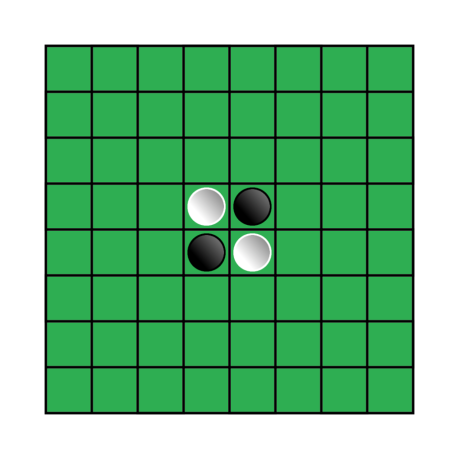
\includegraphics[width=\textwidth]{images/startposition}
    \end{subfigure}%
    \begin{subfigure}{.25\textwidth}
        \caption{White captures}
        \label{fig:othello-capture}
        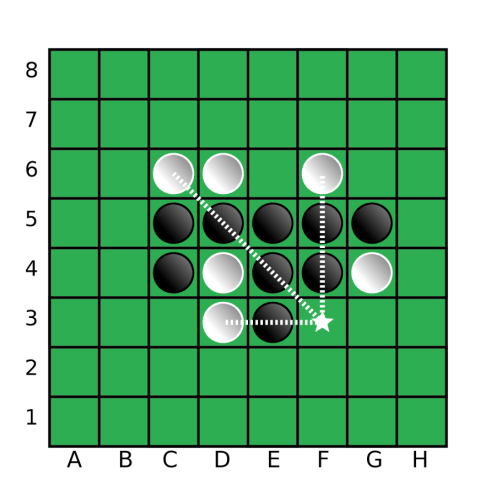
\includegraphics[width=\textwidth]{images/capture}
    \end{subfigure}
    \caption{Uncheckered 8x8 boards}
\end{figure}
\begin{figure}[H]
    \centering
    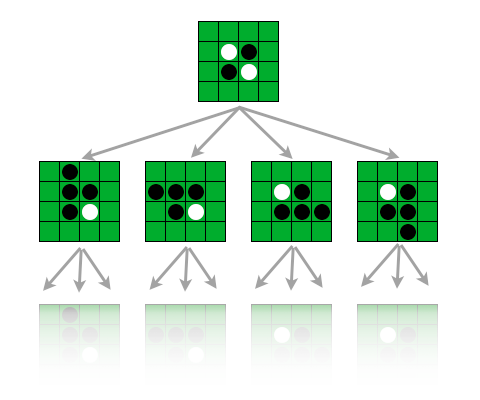
\includegraphics[width=0.4\textwidth]{images/othello-gametree}
    \caption{Othello tree representation}
    \label{fig:othello-gametree}
\end{figure}
\subsection{Othello}
Othello is a strategy board game for two players. Sometimes also referred to as Reversi. Players are assigned a color and take turns placing pieces on the board while capturing pieces of the other player. The player with most pieces left at the end of the game wins.
\subsubsection{Board and moves}
Othello is played on a 8x8 checkered board. It always has the same starting position, see figure: \ref{fig:othello-startposition}. A move is done by placing a piece on an empty square and capturing at least one piece of the opponent in the process. A piece is captured when it becomes surrounded by the other color, see figure: \ref{fig:othello-capture}. When white places a piece on F3. Five pieces get captured and turn white.
\subsubsection{Importance of different squares} The pieces in the middle of the board might be captured and recaptured multiple times, because they are surrounded by so many different positions but the corner squares will never be captured once initially filled, because they cannot be surrounded, making it a safe and valuable position to take. We would expect an algorithm to take advantage of this.
\subsubsection{Game results} The winner of the game is determined by the player with the most pieces at the end of the game. The game ends is when no other available moves are left, this might happen before all the squares are filled, because you may only place a piece if you capture at least one other. It does not matter by how many pieces you you beat the opponent.

\subsection{Tree search}
A game of Othello can be represented as a tree structure where each node represents the state of the board and each edge a valid placement of a new piece that can be taken to transition from one node to the other. See figure \ref{fig:othello-gametree}. Leafs in the tree represent terminating states, when no player can make a valid move. Tree structures like these can be called game trees. Searching through these game trees and finding an optimal or nearly optimal move to make can be achieved via different algorithms. In Othello the depth of a tree is limited, it can not be any bigger than 60, because only one piece is played per move and there are 60 empty squares. The breadth 

\subsection{Minimax tree}
Minimax is a way to search through a game tree and find a good action in a turn based game such as Othello. It works under the assumption that the opponent will always try to win by making optimal moves (minimizing the score of the player while maximizing its own). Figure \ref{fig:mcts-gametree-values} shows a game tree with values per node. The values for each node indicate how well this node is for the players. In fig \ref{fig:mcts-gametree-values} the white nodes indicate that it's the first player's turn to move, the gray nodes are when it is the second player's turn. Player 1 will choose actions that will maximize it's own score, while player 2 will choose actions that minimizes the score of player 1.

\begin{algorithm}
\caption{Monte Carlo Tree Search}
\label{algo:mcts}
\begin{algorithmic}
\Function{MonteCarloPlanning}{rootNode}
\While{no timeout}
\State $leafNode \gets \Call{Select}{rootNode}$
\State $(action, newNode) \gets \Call{Expand}{leafNode}$
\State $reward \gets \Call{Simulate}{newNode}$
\State $ancestors \gets \Call{getAncestors}{newNode}$
\State \Return \Call{UpdateValue}{ancestors}
\EndWhile
\State \Return \Call{bestAction}{state, 0}
\EndFunction
\end{algorithmic}
\end{algorithm}
\subsubsection{Monte Carlo Tree Search}
For a lot of problems the state space is too large to be able to generate and search through the whole game tree. This is also the case with Othello. One approach that works well is to do a simulation step sometimes called a rollout. This simulation step will very quickly and in usually a stochastic manner finish the game, for instance by making random moves until the game ends. The evaluation of this simulation will be used to update the parent nodes in the tree. This is the basic idea behind Monte Carlo Tree Search (MCTS).

MCTS, see algorithm: \ref{algo:mcts}, can be split up in four parts:

\begin{figure}
    \centering
    \begin{subfigure}{0.23\textwidth}
    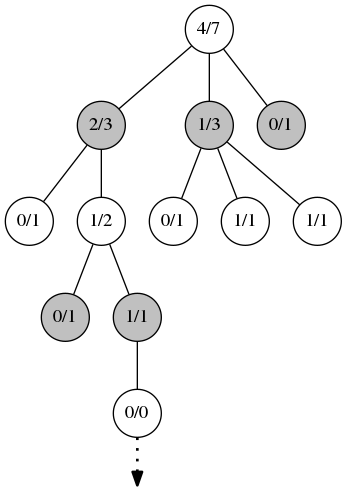
\includegraphics[width=\textwidth]{images/gametree-values}
    \caption{Game tree with values.}
    \label{fig:mcts-gametree-values} 	
    \end{subfigure}%
    \unskip\ \vrule\
    \begin{subfigure}{0.23\textwidth}
    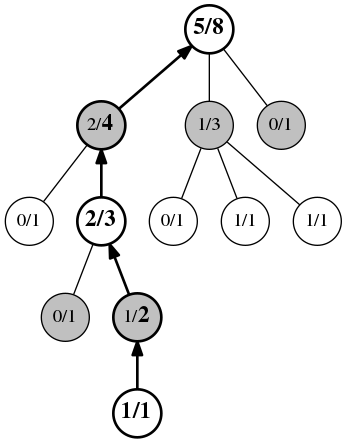
\includegraphics[width=\textwidth]{images/gametree-values-updated}
    \caption{Game tree with  updated values after win.}
    \label{fig:mcts-gametree-values-updated}
    \end{subfigure}
    \caption{MCTS Minimax game tree}
\end{figure}
\begin{enumerate}
    \item SELECT, in this step the algorithm will find a node with an action that has not been investigated yet.
    \item EXPAND, using the node and an action that has not been investigated this step will expand the tree and add a new node.
    \item SIMULATE, Using the new node this step will perform a (fast) simulation of how the game might finish from that point on. For example by taking random actions until the game is over. Note that states generated in the simulation will not be stored or added to the tree. We're only interested in the final evaluation, has player 1 won or lost.
    \item UPDATEVALUE, updating the values for each node is important to actually make the final decision as to which action we will take. Figure \ref{fig:mcts-gametree-values} shows an example game tree. The numbers indicates how many simulations resulted in a player 1 win and how many have been simulated in. Figure \ref{fig:mcts-gametree-values-updated} shows we update each node. 
\end{enumerate}
Lai and Robbins (1985)\cite{Lai+Robbins:1985} showed, for certain reward distributions, logarithmic regret is the best any policy can do.


\textbf{TODO}
\pagebreak[4]
\subsection{Implementation details}
\subsubsection{Testrun}
Wat verstaan wordt onder een test run, meerdere games, wisselend wie er begint
\subsubsection{Domain knowledge in simulation}
Uitleg hoe domain knowledge in de simulation stage toevoegt. welke ik heb toegevoegd. Refereren naar Experiments with Monte Carlo Othello - Philip Hingston en Martin Masek - Edith Cowan Uni
\subsubsection{Genetic Algorithm}
Grove uitleg en hoe ik deze geimplementeerd heb

\begin{figure}
    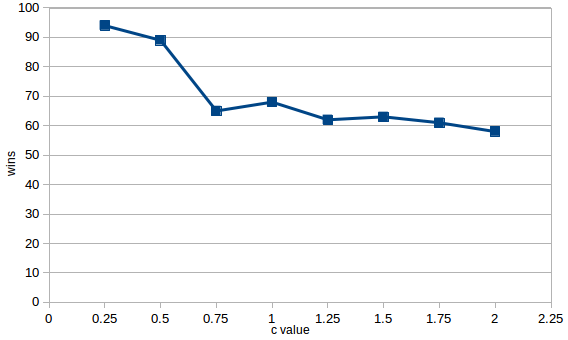
\includegraphics[width=0.5\textwidth]{images/rank-fixed-c-values}
    \caption{Results of having the c values: 0.25, 0.75, 1, 1.25, 1.5, 1.75, 2 compete against each other.}
    \label{fig:results-fixed-rank}
\end{figure}
\begin{figure*}
    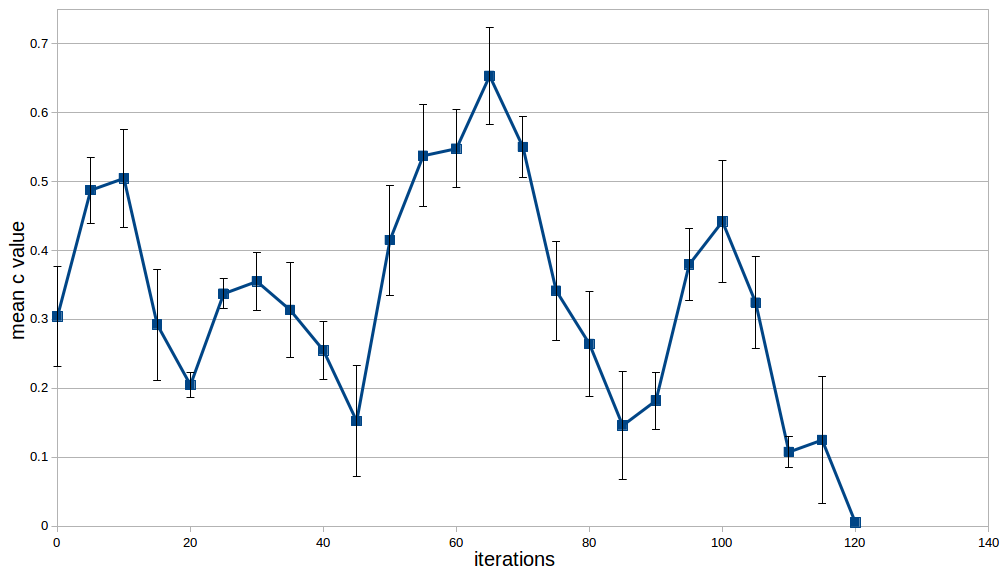
\includegraphics[width=\textwidth]{images/evo-search}
    \caption{Results of having the evolutionary search for a population of c values versus a 0.25 value. On the y axis is the mean c value of the population, the error bars show the variance.}
    \label{fig:results-evo-search}
\end{figure*}

\subsection{Results}
Uitleg van hoofdvraag, rode draad via deelvragen naar hoe zij een antwoord geven op de hoofdvraag
\subsubsection{Is there a significant difference between values}

A pool of 7 distinct values has been tested, the pool consisted of: $\{0.25, 0.75, 1, 1.25, 1.5, 1.75, 2\}$. A total of 420 games have been played amongst them, each two c values played each 20 times. Figure \ref{fig:results-fixed-rank} shows decline in wins the higher the value gets.
\subsubsection{Search for optimal c value}

An evolutionary algorithm (see section: Implementation details) was used to further the search for optimal values. Because figure \ref{fig:results-fixed-rank} showed lower values perform better when competing against higher values the initial population was randomly chosen in the $[0.1, 0.4]$ interval and they all competed against a player using 0.25 as it's c value. Figure \ref{fig:results-evo-search} shows pretty erratic behaviour around the 0.25 - 0.3 value.
\subsubsection{Search for optimal c value in a related problem}
uitleg + resultaat - het probleem iets aanpassen door simulatie met domain knowledge
\subsubsection{optimal c value compared to ucb1-tuned}
MOGELIJK WEGHALEN - heuristiek om exploratie vs exploitatie te regelen, ucb1-tuned

\subsection{Discussion}
Is het significant? en in welke mate? Loont het om moeite te stoppen in het vinden van een optimale c



\printbibliography

\end{document}
